\chapter{Extra Stuff}
\blindtext



\section{Spacing \& Type}
\label{sec:section}

This is a section. This is a citation without brackets. and this is one with brackets \cite{A}. Multiple \cite{A,B,C} Here's a reference to a subsection: \ref{sec:subsection}. The body of the text and abstract must be double-spaced except for footnotes or long quotations. Fonts such as Times Roman, Bookman, New Century Schoolbook, Garamond, Palatine, and Courier are acceptable and commonly found on most computers. The same type must be used throughout the body of the text. The font size must be 10 point or larger and footnotes\footnote{This is a footnote.} must be two sizes smaller than the text\footnote{This is another footnote.} but no smaller than eight points. Chapter, section, or other headings should be of a consistent font and size throughout the ETD, as should labels for illustrations, charts, and figures.  

\subsection{Creating a Subsection}
\label{sec:subsection}

\subsubsection{Creating a Subsubsection}

\paragraph{This is a heading level below subsubsection}

And this is a quote: 
%
\begin{quote}
\blindtext
\end{quote}

This is a table:
% currsize is not set in the long table environment, so we need to set it before we set it up.
\makeatletter
\let\@currsize\normalsize
\makeatother

% tabular environments are set to be single-spaced in the  thesis class,  but long tables do not use tabular
% to get around this, set the spacing to single spacing at the start of the long table environment, and set it back to double-spacing at the end of it

\begin{longtable}{cc}
\caption[This is the title I want to appear in the List of Tables]{This is a caption.} \label{tab:pfams} \\
\hline
A & B \\
\hline
\endfirsthead
\multicolumn{2}{@{}l}{\textbf{Table \thetable} \ldots continued} \\
\hline
A & B \\
\hline
\endhead
a1 & b1 \\
a2 & b2 \\
a3 & b3 \\
a4 & b4 \\
\hline
\end{longtable}





The package ``upgreek'' allows us to use non-italicized lower-case greek letters. See for yourself: $\upbeta$, $\bm\upbeta$, $\beta$, $\bm\beta$. Next is a numbered equation:
\begin{align}
\label{eq:name}
\|\bm{X}\|_{2,1}={\underbrace{\sum_{j=1}^nf_j(\bm{X})}_{\text{convex}}}=\sum_{j=1}^n\|\bm{X}_{.,j}\|_2
\end{align}
The reference to equation (\ref{eq:name}) is clickable. 



\section{Figure and Graphic} 

The experiment as shown in Fig.\ref{fig:exp02}, demonstrates a long range of motion with a high conditional number. In this trajectory, the highest conditional number hits up to 2900. However, the result shows that the state error and controller cost are relatively small as shown in table \ref{tab:pfams}.


\begin{figure}[H]
\begin{subfigure}{.5\textwidth}
  \centering
  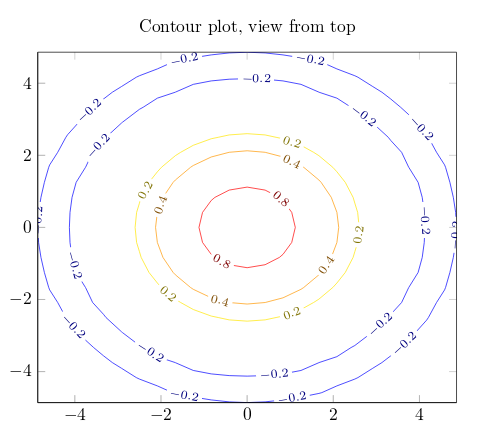
\includegraphics[width=.8\linewidth]{figs/contour.png}
      \caption{Initial position}
  \label{fig:traj2}
\end{subfigure}%
\begin{subfigure}{.5\textwidth}
  \centering
  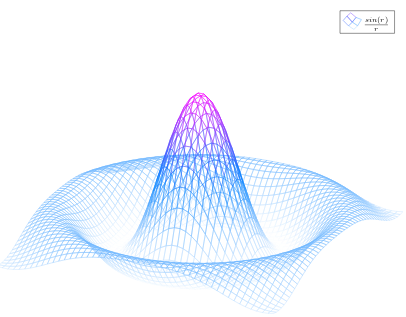
\includegraphics[width=.8\linewidth]{figs/mesh.png}
      \caption{Final position}
  \label{fig:traj1}
\end{subfigure}
\caption{Long range motion: line trajectory}
\label{fig:exp02}
\end{figure}


\begin{figure}[H]
\begin{subfigure}{.5\textwidth}
  \centering
  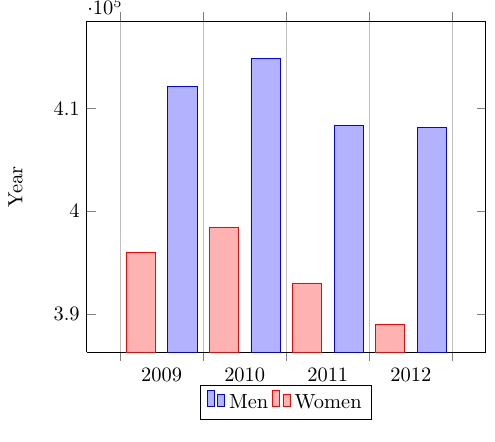
\includegraphics[width=1\linewidth]{figs/Plot.png}
      \caption{Reference and actual state}
  \label{fig:x2}
\end{subfigure}%
\begin{subfigure}{.5\textwidth}
  \centering
  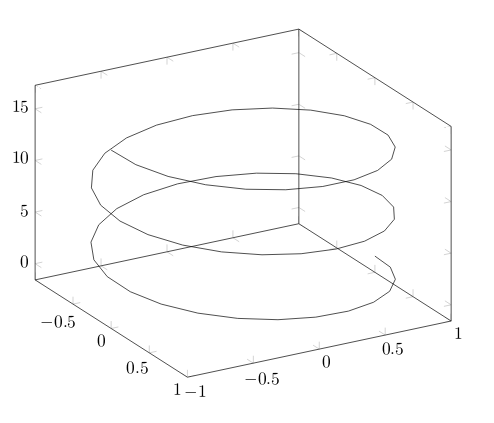
\includegraphics[width=1\linewidth]{figs/spiral.png}
      \caption{State error between actual and referent}
  \label{fig:e_x2}
\end{subfigure}
\caption{State tracking of long range motion(line trajectory)}
\label{fig:x1_ex2}
\end{figure}




\section{Flowchart}

The following example contains the code and can be opened directly in \href{https://www.overleaf.com/learn/latex/LaTeX_Graphics_using_TikZ%3A_A_Tutorial_for_Beginners_(Part_3)%E2%80%94Creating_Flowcharts}{Overleaf}. This code adds the option trapezium stretches=true to the node style definition, helping to ensure trapezium nodes are the same width.

\begin{tikzpicture}[node distance=2cm]

\node (start) [startstop] {Start};
\node (in1) [io, below of=start] {Input};
\node (pro1) [process, below of=in1] {Process 1};
\node (dec1) [decision, below of=pro1, yshift=-0.5cm] {Decision 1};

\node (pro2a) [process, below of=dec1, yshift=-1.5cm] {Process 2a
text text text text
text text text};

\node (pro2b) [process, right of=dec1, xshift=3cm] {Process 2b};
\node (out1) [io, below of=pro2a, yshift=-0.5cm] {Output};
\node (stop) [startstop, below of=out1] {Stop};

\draw [arrow] (start) -- (in1);
\draw [arrow] (in1) -- (pro1);
\draw [arrow] (pro1) -- (dec1);
\draw [arrow] (dec1) -- node[anchor=east] {yes} (pro2a);
\draw [arrow] (dec1) -- node[anchor=south] {no} (pro2b);
\draw [arrow] (pro2b) |- (pro1);
\draw [arrow] (pro2a) -- (out1);
\draw [arrow] (out1) -- (stop);

\end{tikzpicture}



\section{Algorithm and pseudo code}

Here we demonstrate how algorithms or pseudocode can be typeset using the \verb|algorithmic| environment provided by the \verb|algpseudocode| package.



\begin{algorithm}
\caption{Example While Loop}
\begin{algorithmic}[1]
\State $i \gets 0$
\While{$i < 10$}
    \State Print $i$
    \State $i \gets i + 1$ \Comment{This is a comment}
\EndWhile
\end{algorithmic}
\end{algorithm}


\section{Code Display}

Example of display of your code. 

\begin{lstlisting}[language=Python]
# This is a black comment
def hello():
    print("Hello, world!")  # Keyword 'def' is blue, comment is black
\end{lstlisting}





\section[Theorems, Corollaries, Lemmas, Proofs, Remarks, Definitions and Examples]{Theorems, Corollaries, Lemmas, Proofs, Remarks, Definitions,and Examples}

\begin{theorem}
\label{thm:onlytheorem}
\blindtext
\end{theorem}

\begin{proof}
I'm a (very short) proof.
\end{proof}

\begin{lemma}
I'm a lemma.
\end{lemma}

\begin{corollary}
I include a reference to Thm. \ref{thm:onlytheorem}.
\end{corollary}

\begin{proposition}
I'm a proposition.
\end{proposition}

\begin{remark}
I'm a remark. 
\end{remark}

\begin{definition}
I'm a definition. I'm a definition. I'm a definition. I'm a definition. I'm a definition. I'm a definition. I'm a definition. I'm a definition. I'm a definition. I'm a definition. I'm a definition. 
\end{definition}

\begin{example}
I'm an example.
\end{example}


\section[Optional table of contents heading]{Section with\\ linebreaks in\\the
name}


\Blindtext[2]


\chapter{Even More Extra Stuff}
\blindtext